\documentclass[a4paper,12pt]{article}
\usepackage[utf8]{inputenc}
\usepackage[polish]{babel}
\usepackage[T1]{fontenc}
\usepackage[lmargin=2cm,rmargin=2cm]{geometry}
\usepackage{graphicx}
\usepackage{float}
\usepackage{longtable}
\usepackage{hyperref}
\title{System wspomagający pracę ratowników górskich Babiej Góry}
\author{Arkadiusz Błasiak, Szymon Nowak}
\date{}
\begin{document}
\maketitle
\tableofcontents
\newpage
\section{Cel}
System ma na celu wspomagać pracę ratowników górskich Babiej Góry. Dokładne informacje o warunkach pogodowych i lokalizacje pobierane z BTS’ów, pomogą ratownikom monitorować szlaki z większą dokładnością, przyspieszyć czas reakcji oraz podjąć decyzję o rozpoczęciu akcji ratunkowej.
\section{Narzędzia}
Do stworzenia aplikacji został wykorzystany framework webowy \textbf{Django} oraz język Python. Przesyłanie komunikatów między nadajnikami a serwerem realizowane jest za pomocą brokera wiadomości \textbf{Apache Kafka}.
\section{Konfiguracja}
\begin{enumerate}
\item Wykonaj kroki 1 oraz 2 z sekcji "Quick Start" według instrukcji na stronie \url{http://kafka.apache.org/documentation.html#quickstart}
\item Zainstaluj Pythona 2.7 \url{https://www.python.org/download/releases/2.7/}
\item Zainstaluj menedżer pakietów Pythona -- pip \url{https://pip.pypa.io/en/stable/installing/}
\item Będąc w katalogu z projektem, zainstaluj wymagane pakiety za pomocą polecenia \textit{pip install -r requirements.txt}
\item Uruchom serwer za pomocą polecenia \textit{python manage.py runserver 0.0.0.0:8000}
\item Serwer zostanie uruchomiony na porcie 8000, wpisz w przeglądarce \url{http://localhost:8000} aby wejść do aplikacji
\item Uruchom odbiorniki -- użyj polecenia \textbf{python odbiornikN.py \&}, ampersand sprawi, że proces przejdzie w tło.\\ PAMIĘTAJ! Aby odbiorniki/nadajniki poprawnie funkcjonowały, serwer Apache Kafka musi działać.
\end{enumerate}
\newpage
\section{Podstawowe założenia}
\begin{enumerate}
\item Babia Góra podzielona jest na 11 szlaków o różnej długości i różnym poziomie trudności (żółty, zielony, niebieski, czarny, czerwony). Dla każdego szlaku obliczana będzie skala zagrożenia
\item Na skalę zagrożenia każdego szlaku wpływają:
\begin{itemize}
\item warunki atmosferyczne
\begin{itemize}
\item wiatr
\item deszcz
\item mgła
\item temperatura
\end{itemize}
\item zagrożenie lawinowe
\item poziom trudności szlaku
\end{itemize}
\item Informacje o warunkach atmosferycznych pobierane są z czujników rozmieszczonych w różnych miejscach na szlakach Babiej Góry. Informacje o lokalizacji komórek turystów pobierane są BTS’ów
\item Każdy z powyższych czynników posiada osobną skalę. Końcowy poziom stanu alarmowego dla każdego szlaku oblicza się ze wzoru: (suma skal dla warunków atmosferycznych + zagrożenie lawinowe + poziom trudności szlaku)/4.
\item W zależności od uzyskanego wyniku system sugeruje określone akcje ratowników
\end{enumerate}
\newpage
\section{Szlaki babiej góry}
\begin{center}
    \begin{longtable}{ | l | l | p{5cm} | l | l | p{2cm} |}
    \hline
    \textbf{Lp} & \textbf{Kolor} & \textbf{Trasa} & \textbf{Czas przejścia} & \textbf{Długość trasy} & \textbf{Poziom trudności}\\ \hline
    1 & żółty & Markowe Szczawiny -- Sucha Kotlinka -- Diablak & 1h 30min & 3km & 1\\\hline
    2 & żółty & Zawoja Czatoża -- Fickowe Rozstaje -- Górny Płaj -- Markowe
Szczawiny & 3h 20min & 5km & 1\\\hline
	3 & niebieski & Zawoja Czatoża -- Markowe Rówienki -- Zawoja Markowa --Ryzowana -- Zawoja Policzne & 3h 30min & 7,50km & 2\\\hline
	4 & niebieski & Zawoja Policzne -- Polana rowiarki -- Markowe Szczawiny & 3h & 11km & 2\\\hline
	5 & zielony & Zawoja Markowa -- Pośredni Bór -- Markowe Szczawiny & 1h 20min &  & 3\\\hline
	6 & zielony & Górny Płaj -- Sokolica & 45min & 1,5km & 3\\\hline
	7 & zielony & Przełęcz Jałowiecka -- Mała Babia Góra -- Przełęcz Brona & 2h & 4km & 3\\\hline
	8 & zielony & Przywarówka -- Głodna Woda -- Diablak & 2h 30min & 2,3km & 3\\\hline
	9 & zielony & Polana Krowiarki -- Hala Śmietanowa -- Zubrzyca Górna & 2h & 3km & 3\\\hline
	10 & czerwony & Polana Krowiarki -- Sokolica -- Kępa -- Gówniak -- Diablak -- Przełęcz Brona -- Markowe Szczawiny -- Fickowe Rozstaje -- Przełęcz Jałowiecka & 6h & 14,5km & 4\\\hline
	11 & czarny & Podryzowana -- Ryzowana -- Markowe Szczawiny & 2h 30min & 3,5km & 4\\\hline
    \end{longtable}
\end{center}
\newpage
\section{Czynniki atmosferyczne}
\begin{center}
    \begin{longtable}{ | l | p{5cm} | l | l |}
    \hline
    \textbf{Czynnik} & \textbf{Opis} & \textbf{Skala} & \textbf{Wytyczne} \\ \hline
    wiatr & Przy wietrze o prędkości 80–100
km/godz trudno utrzymać się na nogach
pokonywanie wysokogórskich szlaków
jest często niemożliwe, grozi
przewróceniem lub wręcz
zdmuchnięciem w przepaść. Poruszając
się w terenach leśnych, narażamy się na
przygniecenie przez łamane wiatrem i
wywracające się drzewa lub uderzenie
spadającymi gałęziami. &
1--3 & \parbox[t]{5cm}{1: do 30km/h\\
2: 30-80km/h\\
3: powyżej 80km/h} \\ \hline
	mgła&Jej obecność może nie tylko
uniemożliwić oglądanie widoków, ale przede wszystkim znacznie utrudnić
orientację w terenie. Szczególnie
niebezpieczna jest mgła w warunkach
zimowych, gdy biel śniegu całkowicie
zlewa się z bielą mgły. Nie widząc
punktów odniesienia, nie będziemy w
stanie określić położenia w terenie,
kierunku marszu, a nawet ocenić
stromizny stoku, na którym się
znajdujemy.& 1--3 & \parbox[t]{5cm}{1: zauważalna
mgła, która nie wpływa jednak na
poruszanie się po
szlaku\\
2: słaba widoczność\\
3: znikoma
widoczność,
znaczące
utrudnienia w
orientacji
terenowej} \\ \hline
 	temperatura & Na szczytach temperatura z reguły jest
niższa niż u stóp gór. Każde 100 metrów
wyżej, to około 1 st. C mniej. Uczucie
zimna jest dodatkowo potęgowane przez
wiatr. Słaby wiaterek przy termometrze
wskazującym zero stopni spowoduje
odczuwanie zimna równe około 3 st. 
C,
podmuch (5 m/s) – prawie 9 st. 
C, wiatr 15
m/s aż 18 st.
C. Ten sam wiatr przy
umiarkowanym mrozie 10 st.
C da
odczucie poniżej 33 st.
C. & 1--3 & \parbox[t]{5cm}{1: powyżej 15 lub
poniżej 5\\
2: powyżej 24 lub
poniżej -3\\
3: powyżej 30 lub
poniżej -15}\\ \hline
	deszcz, burza & W górach jest niebezpieczne podczas
burzy ze względu na ilość dni burzowych
w ciągu roku, wysokość brak
możliwości schronienia się. Dodatkowym
zagrożeniem są barierki, łańcuchy,
drabiny, brak dobrze przewodzacych
warstw. Burza jest niebezpieczna, jeżeli
pomiędzy błyskiem a grzmotem jest
mniej niz 515
sekund. Znaczy to, że
piorun uderzył bliżej niż 25
km od nas.
Dodatkowo opady deszczu podwyższają
trudności tras związane z poruszaniem
sie po nich. & 1--3 & \parbox[t]{5cm}{1:
deszcz - od 15 do
40mm
wiatr - od 0 do
30km/h\\
2:
deszcz - od 41 do
70mm
wiatr - od 31 do
80kmh\\
3:
deszcz - powyżej
70mm
wiatr - powyżej
80kmh}\\ \hline
    \end{longtable}
\end{center}
\newpage
\section{Zagrożenie lawinowe}
\begin{center}
    \begin{longtable}{ | l | p{10cm} |}
    \hline
    \textbf{Stopień zagrożenia} & \textbf{Prawdopodobieństwo zejścia lawiny}\\ \hline
    5 & Istnieje prawdopodobieństwo samoczynnego schodzenia wielu dużych, niejednokrotnie
również bardzo dużych lawin, także w terenie
umiarkowanie stromym. \\\hline
	4 & Wyzwolenie lawiny jest prawdopodobne na
licznych stromych stokach już przy małym
obciążeniu dodatkowym. W niektórych
przypadkach możliwe jest samorzutne
schodzenie licznych średnich, a często
również dużych lawin.\\\hline
	3 & Wyzwolenie lawiny jest możliwe już przy
małym obciążeniu dodatkowym wszystkim na
wskazanych stromych stokach. W niektórych
przypadkach możliwe jest samorzutne
schodzenie średnich, a sporadycznie także
dużych lawin.\\\hline
	2 & Wyzwolenie lawiny jest możliwe zwłaszcza
przy dużym obciążeniu dodatkowym przede
wszystkim na wskazanych stromych stokach.
Nie należy spodziewać się samorzutnego
schodzenia dużych lawin.\\\hline
	1 & Wyzwolenie lawiny na ogół jest możliwe tylko
przy dużym obciążeniu dodatkowym w
nielicznych miejscach w terenie ekstremalnie
stromym. Możliwe jest samorzutne schodzenie
lawin głównie w postaci zsuwów i małych
lawin. \\\hline
    \end{longtable}
\end{center}
\newpage
\section{Sytuacje alarmowe -- turyści}
\begin{center}
\begin{longtable}{ | p{10cm} | p{5cm} | }
\hline
	\textbf{Sytuacja alarmowa} & \textbf{Kiedy występuje}\\\hline
	Turysta przebywa w jednym miejscu przez
dłuższy czas. Możliwe zasłabnięcie, utracenie
przytomności. & Turysta nie rusza się od 15 minut\\\hline
	Turysta znajduje się w miejscu zabronionym lub
zamknietym ze wzgledu na panujace warunki
atmosferyczne np zagrozenie lawinowe. & Turysta wchodzi na obszar zagrożenia\\\hline
	Turysta oddalił się od grupy. Możliwe zgubienie. & Turysta oddalił się od lidera grupy na >= 200m\\\hline
\end{longtable}
\end{center}
\newpage
\section{Stany alarmowe dla szlaków}
\begin{center}
\begin{longtable}{ | p{4cm} | p{5cm} | p{5cm} | }
\hline
	\textbf{Poziomy stanu alarmowego} & \textbf{Zalecenia dla ruchu osób} & \textbf{Zalecane działania ratowników} \\\hline
	1 -- niski & Na ogół dogodne warunki dla
wędrówek. & System monitoruje \\\hline
	2 -- umiarkowany & Częściowo niekorzystne warunki.
Poruszanie się wymaga
umiejętności oceny lokalnego
zagrożenia lawinowego i
odpowiedniego wyboru trasy
szczególnie na wszystkich
stromych stokach, oraz na
stokach średnio stromych
szczególnie wskazanych pod
względem wystawy i wysokości. & Monitorowanie turystów
na zagrożonych
obszarach. \\\hline
 3 -- znaczny & Warunki w znacznej mierze
niekorzystne. Poruszanie się
wymaga bardzo dużego
doświadczenia. & Wysłanie drona w celu
lepszego monitorowania
szlaku. \\\hline
4 -- wysoki & Warunki zdecydowanie
niekorzystne. Poruszanie się
wymaga ekstremalnie dużej
wprawy i doświadczenia. Zaleca
się zaniechanie wszelkich wyjść
w góry. & Wysłanie drona do
zbadania sytuacji i
podjęcia decyzji o
wysłaniu ekipy
ratowniczej. \\\hline
5 -- bardzo wysoki & Poruszanie się w terenie jest
zazwyczaj niemożliwe. Zaleca się
zaniechanie wszelkich wyjść w
góry. & Przechwycenie turystów \\\hline
\end{longtable}
\end{center}
\section{Rozmieszczenie BTSów w pobliżu Babiej Góry}
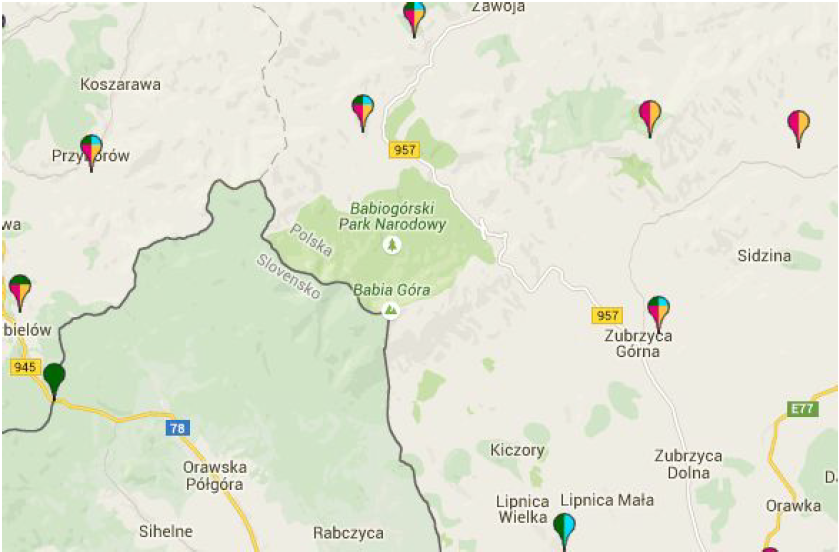
\includegraphics[scale=0.75]{bts.png}
\newpage
\section{Określanie pozycji komórki}
TA – Czas jaki pokonuje sygnał pomiedzy komorka a stacja BTS , zwykle 0-63\\
RxL – Siła sygnału, zwykle 0110dBm
aktualny poziom sygnału odbieranego ze stacji do której jesteśmy zalogowani.
przyklady: 71\% 103dBm,
80\% 89dBm\\
TxPwr – poziom mocy, zwykle 0~19 dBm\\
A,B - A
to współczynnik tłumienia sygnału RF,B to współczynnik transmisji tłumienia mocy\\
RF częstotliwość
drgań elektromagnetycznych stosowanych w szeroko rozumianej
radiotechnice. W zakres częstotliwości radiowych wchodzą drgania o zakresie od 3 kHz do
300 GHz.\\
\textbf{Distance(L)=TA*500+RxL*A+TxPwr*B} -- odległość komórki od konkretnego
BTS\\
potrzebna współrzędnych z gpsu do określenia pozycji stacji bts\\
po określeniu odległości, nakreślamy okrąg dookoła btsu na którym znajduje się komórka\\
przy danych z 3 btsow lokalizacja telefonu będzie się znajdować na przecięciu okregów\\
\begin{center}
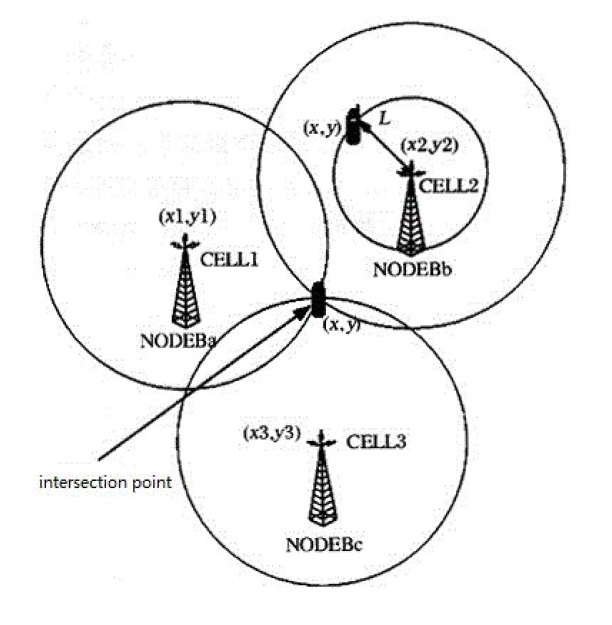
\includegraphics[scale=0.75]{intersection.png}
\end{center}
Dokładność takiego namierzania: od 50 do 550 (im więcej BTSów tym dokładniejsza
pozycja). Dla ułatwienia, w projekcie, nadajnik przesyła dokładne koordynaty GPS komórki.
\newpage
\section{Interfejs użytkownika}
Po wejściu do aplikacji należy się zalogować, domyślny login to \textbf{admin}, a hasło \textbf{adminadmin}. Hasło można zmienić w konsoli za pomocą komendy \textbf{python manage.py createsuperuser}.
\begin{center}
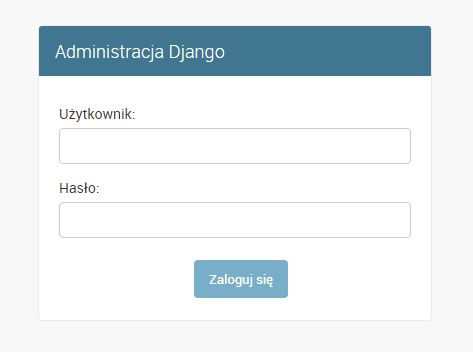
\includegraphics[scale=1]{ui0.png}
\end{center}
\subsection{Główny interfejs}
Główny interfejs wygląda następująco
\begin{center}
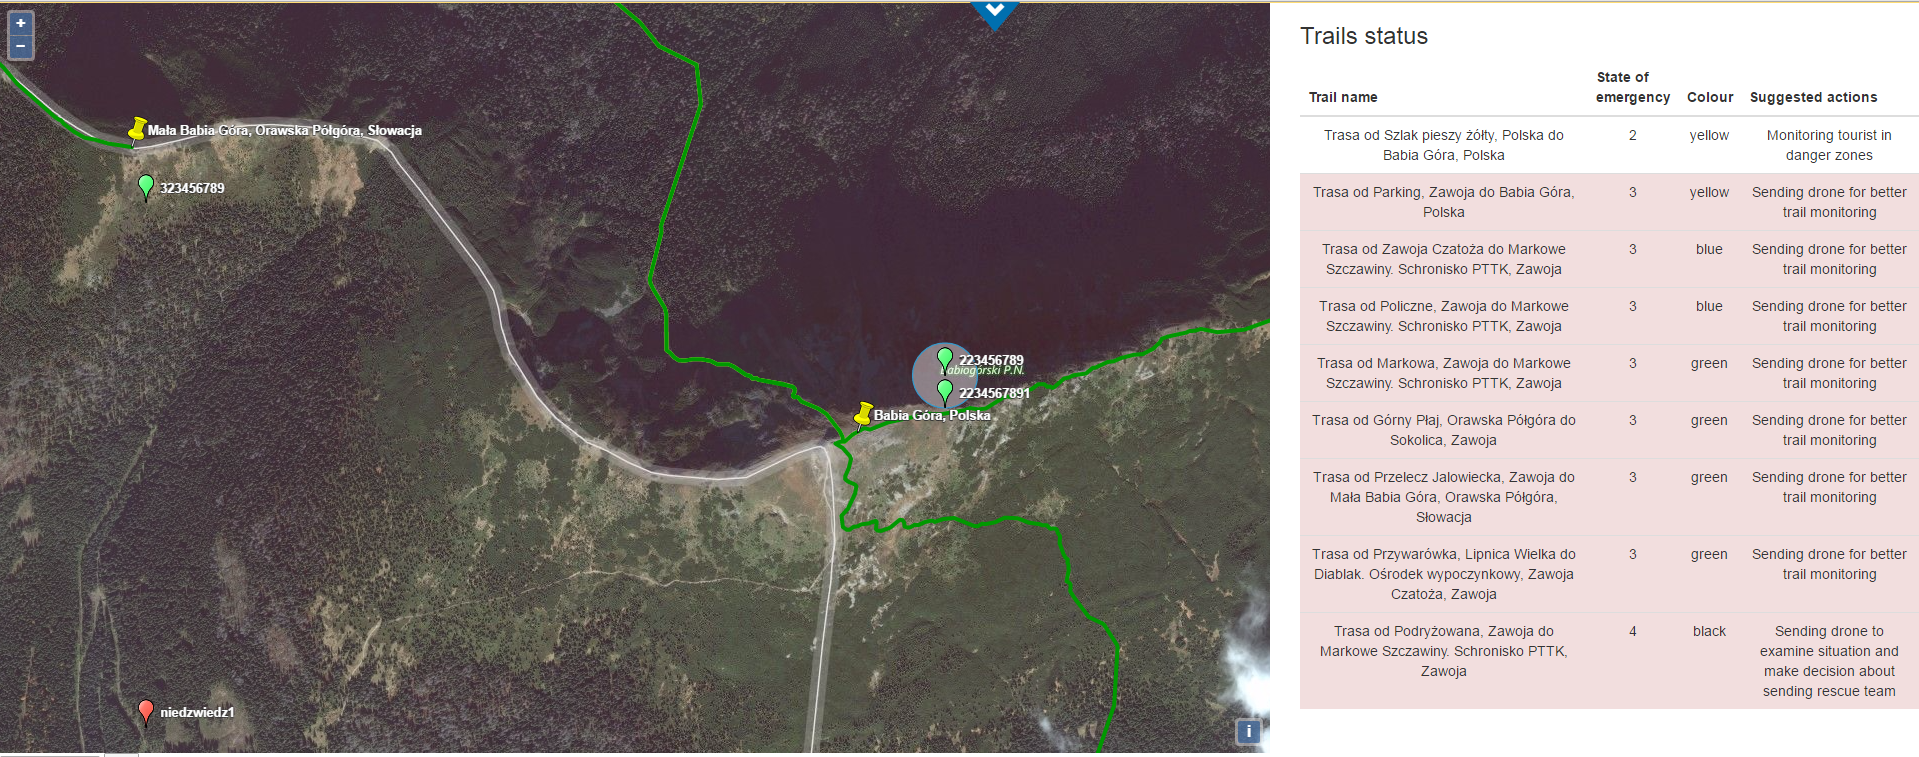
\includegraphics[scale=0.4]{ui1.png}
\end{center}
Po lewej znajduje się mapa z naniesionymi szlakami oraz pozycjami turystów. Żółte pinezki symbolizują punkty końcowe/początkowe szlaków. Zielone kropki to pozycje turystów. Po prawej stronie znajduje się informacja o aktualnym poziomie zagrożenia na poszczególnych szlakach. Jeśli poziom jest wysoki, pozycja zaznaczana jest na czerwono.
\subsection{Menu}
Strzałka u góry rozwija menu
\begin{center}
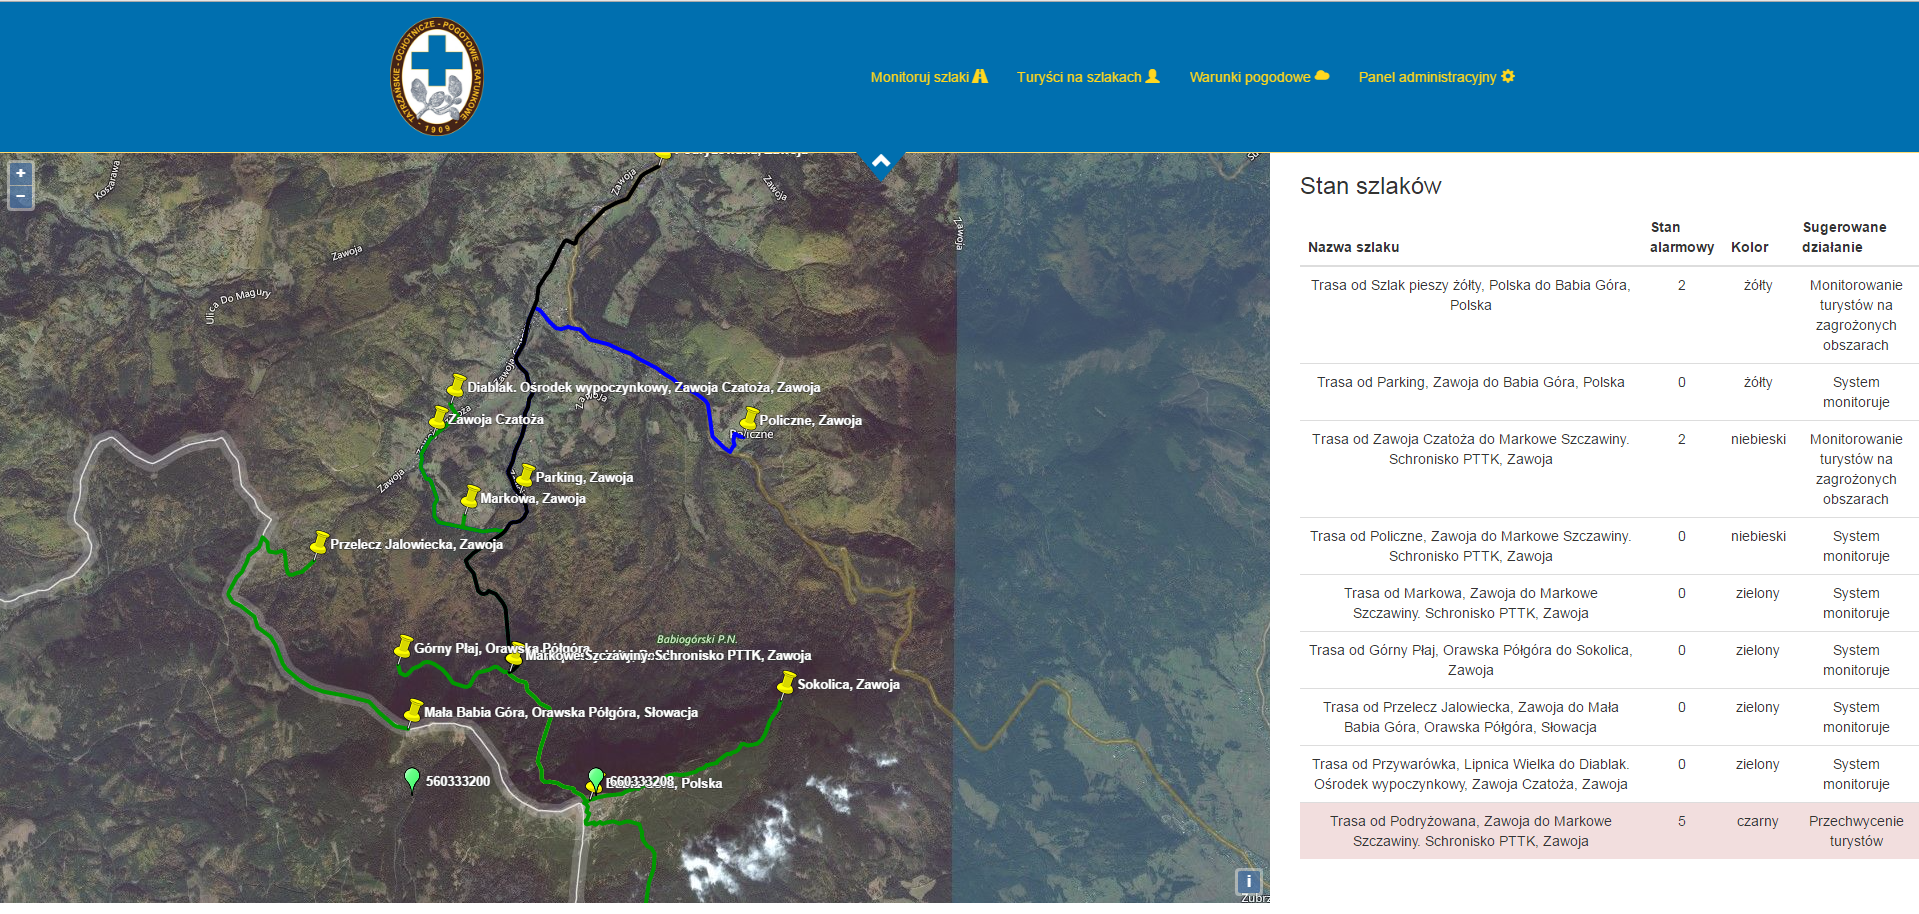
\includegraphics[scale=0.4]{ui2.png}
\end{center}
Dostępne pozycje to
\begin{itemize}
\item Monitoruj szlaki (domyślny widok po zalogowaniu do aplikacji) -- stan szlaków
\item Turyści na szlakach -- monitorowanie czy turystom nic nie grozi
\item Warunki pogodowe -- jaka pogoda panuje na szlakach
\item Panel administracyjny -- zarządzanie systemem (m.in. dodawanie grup, ustawienia szlaków, tworzenie stref zagrożonych)
\end{itemize}
\subsection{Turyści na szlakach}
\begin{center}
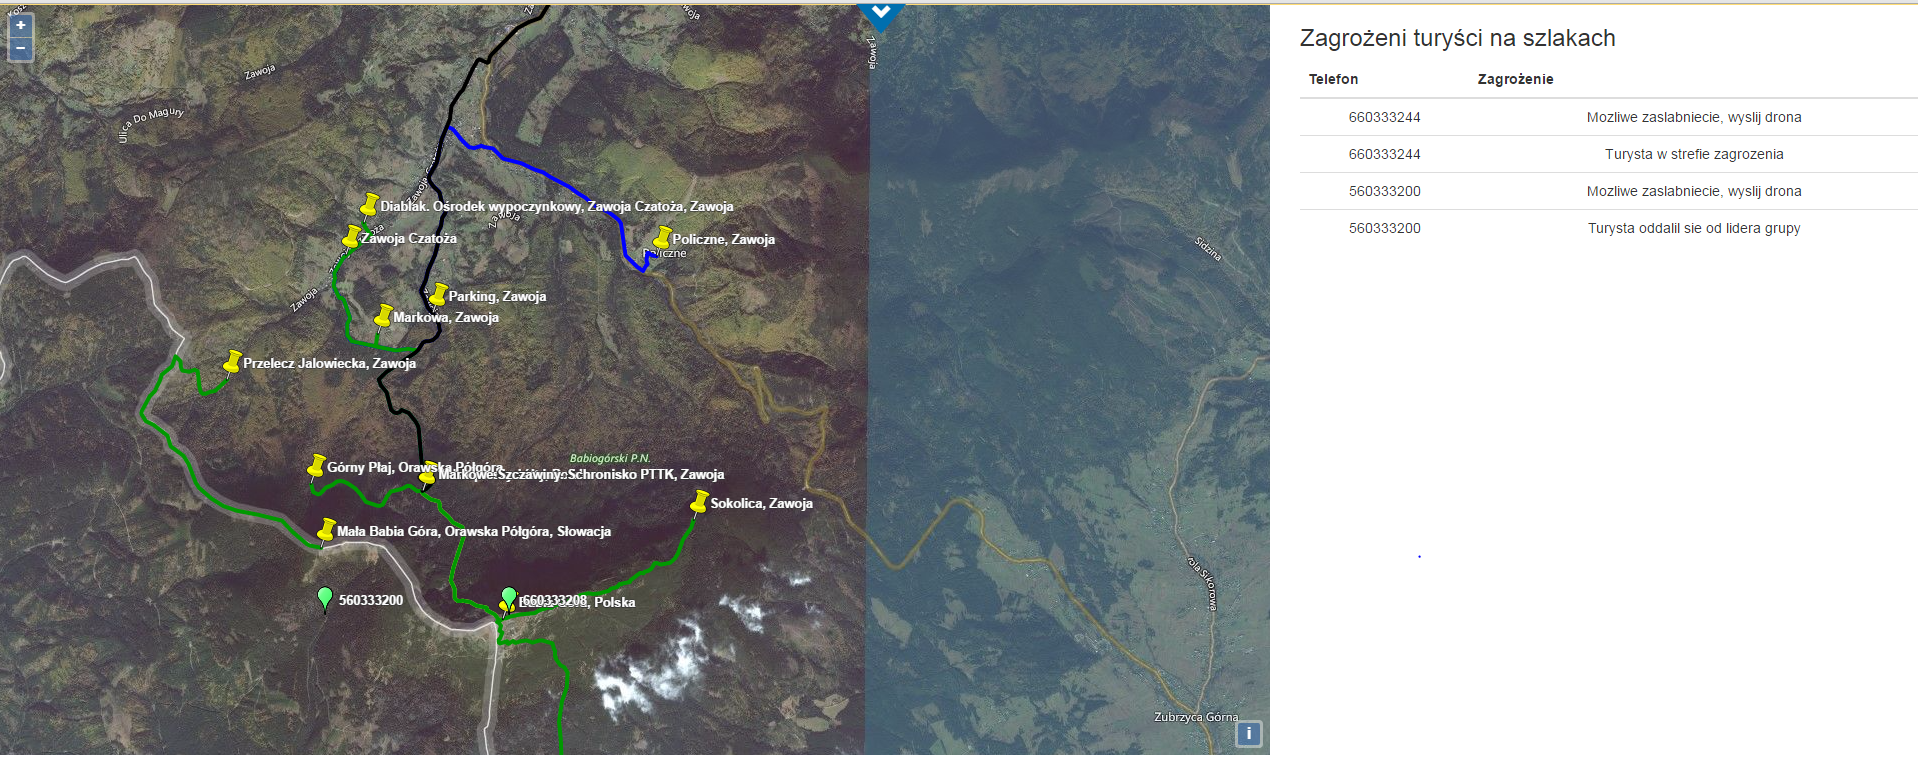
\includegraphics[scale=0.4]{ui3.png}
\end{center}
Po lewej znajduje się mapa z naniesionymi szlakami oraz pozycjami turystów. Żółte pinezki symbolizują punkty końcowe/początkowe szlaków. Zielone kropki to pozycje turystów. Po prawej stronie znajduje się informacja o zagrożonych turystach -- numer telefonu oraz rodzaj zagrożenia.
\subsection{Warunki pogodowe}
\begin{center}
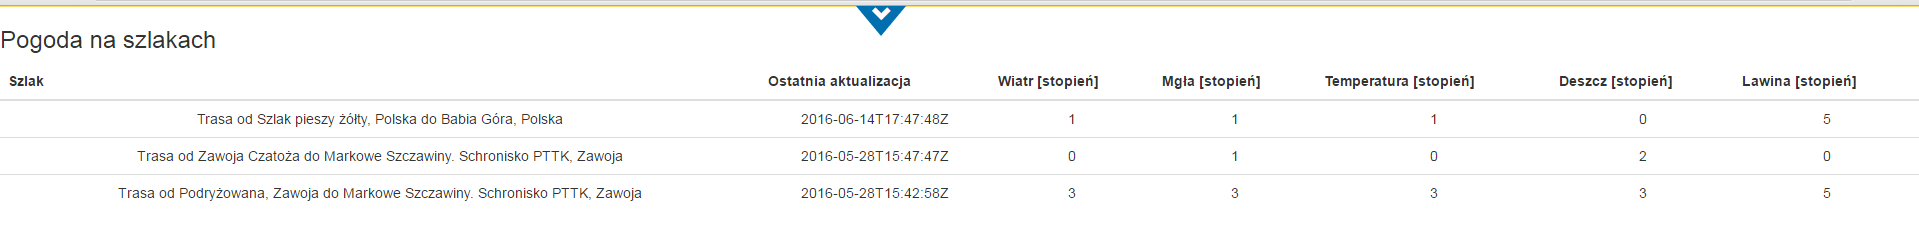
\includegraphics[scale=0.4]{ui4.png}
\end{center}
W tej sekcji pokazane są aktualne warunki pogodowe na szlakach -- nazwa szlaku, ostatnia aktualizacja warunków pogodowych oraz stopnie poszczególnych czynników.
\subsection{Panel administracyjny}
\begin{center}
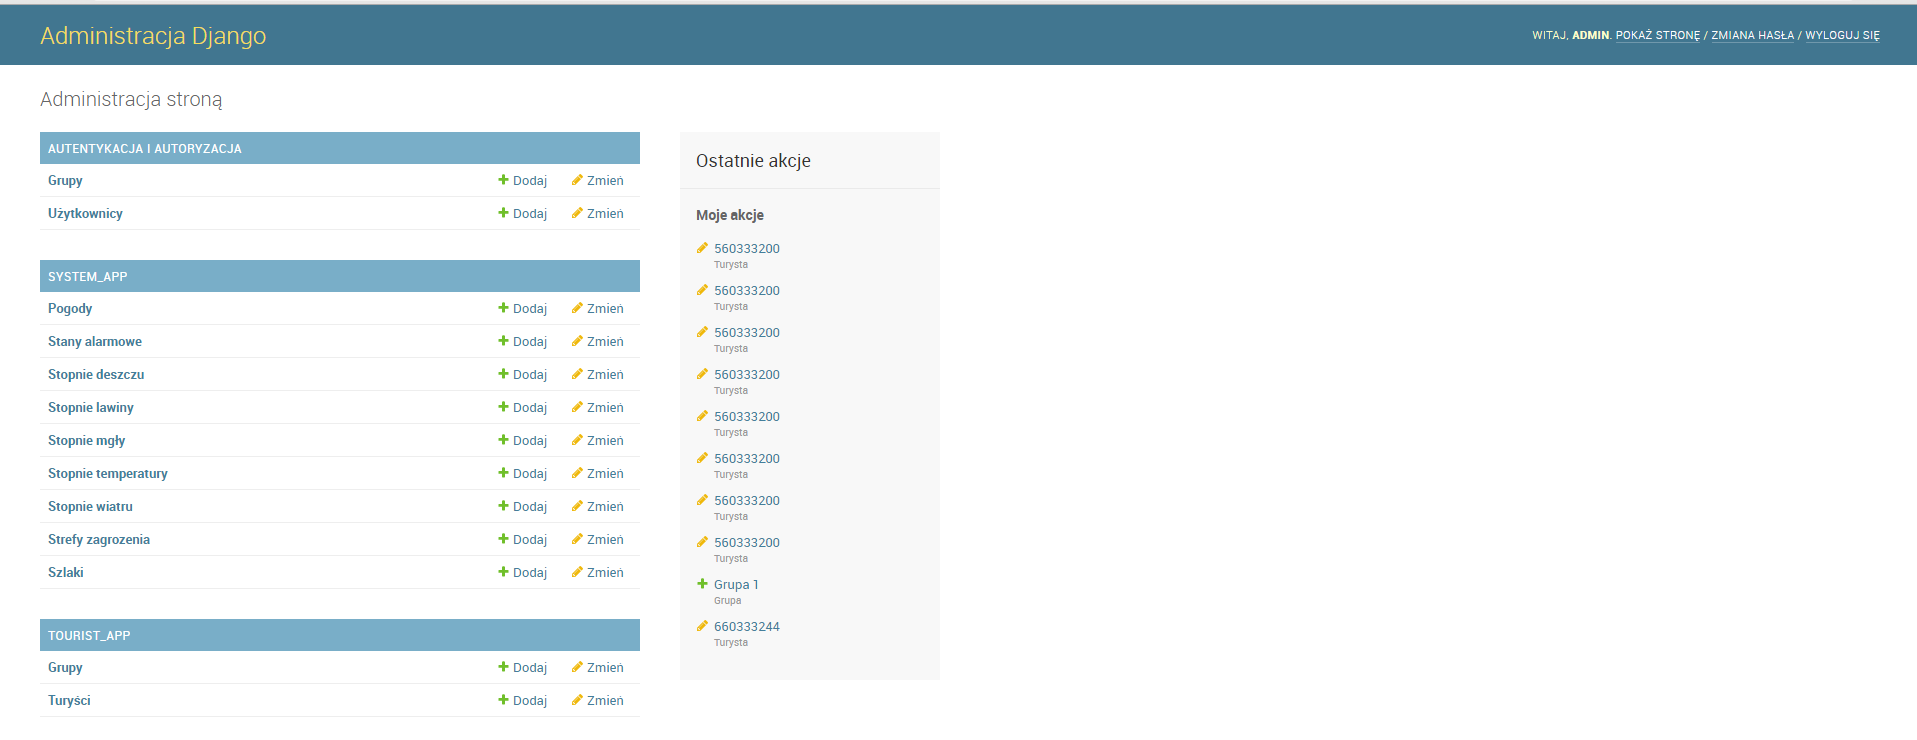
\includegraphics[scale=0.4]{ui5.png}
\end{center}
Najważniejszymi elementami panelu są \textbf{Grupy (TOURIST\_APP)} oraz \textbf{Strefy zagrożenia (SYSTEM\_APP)}. Reszta opcji nie wymaga zmian, jednak gdyby zaszła taka potrzeba, system można dostosować (dodawanie/usuwanie/edycja szlaków, stopni warunków pogodowych, zarządzanie użytkownikami)
\subsubsection{Strefy zagrożenia}
\begin{center}
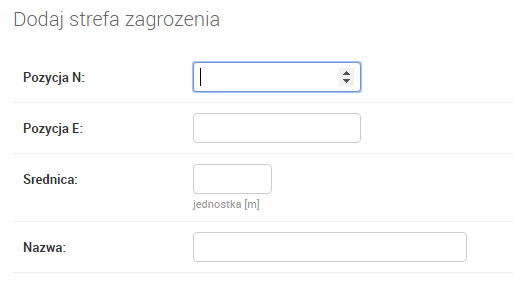
\includegraphics[scale=1]{ui6.png}
\end{center}
W tej zakładce można dodać, edytować oraz usunąć strefy zagrożenia. Aby dodać nową, należy wprowadzić odpowiednie pozycje GPS, promień (strefa zagrożenia jest kołem) oraz nazwę strefy
\subsubsection{Grupy}
\begin{center}
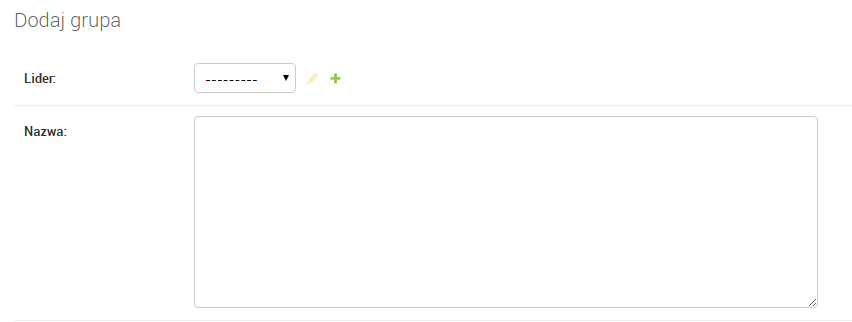
\includegraphics[scale=1]{ui7.png}
\end{center}
W tej zakładce można dodać, edytować oraz usunąć grupy turystów. Aby dodać nową, należy wybrać lidera oraz podać nazwę grupy. Turystów do grupy przyporządkowuje się z zakładki \textbf{Turyści}
\section{Diagram klas}
\begin{center}
\includegraphics[scale=0.5]{klasy.png}
\end{center}
\section{Diagram przypadków użycia}
\includegraphics[scale=0.7]{uc.png}
\section{Diagramy aktywności}
\subsection{Diagram aktywności dla przypadku użycia -- Ustal pozycje turystów}
\begin{center}
\includegraphics[scale=0.56]{da1.png}
\end{center}
\newpage
\subsection{Diagram aktywności dla przypadku użycia -- Sprawdź przytomność turystów}
\includegraphics[scale=0.7]{da2.png}
\newpage
\subsection{Diagram aktywności dla przypadku użycia -- Identyfikuj zagrożenia w obrębie grupy}
\includegraphics[scale=0.7]{da3.png}
\newpage
\subsection{Diagram aktywności dla przypadku użycia -- Identyfikuj turystów w obrębie stref zagrożonych}
\includegraphics[scale=0.7]{da4.png}
\newpage
\subsection{Diagram aktywności dla przypadku użycia -- Oblicz skalę zagrożenia}
\includegraphics[scale=0.56]{da5.png}
\section{Scenariusze}
\subsection{Charakterystyka użytkowników}
\begin{itemize}
\item ID: AKT\_UZ\\
Nazwa: Użytkownik/Kontroler\\
Opis: Użytkownik to osoba częściowo obsługująca aplikację. Wprowadza
część danych i podejmuje końcową decyzję na podstawie zanalizowanych
danych o podjęciu akcji ratunkowej albo wysłaniu drona na zwiad.
\item ID: AKT\_CZ\\
Nazwa: Czujnik\\
Opis: Czujniki przekazują dane atmosferyczne niezbędne do wyliczenia skal
zagrożenia i ustalenia warunków panujących na szlakach i konkretnych
miejscach.
\item ID: AKT\_BTS\\
Nazwa: BTS\\
Opis: Stacje BTS lokalizują na bieżąco pozycje telefonów komórkowych
znajdujących się obszarze Babiej Góry i przekazują współrzędne do aplikacji.
\item ID: AKT\_A\\
Nazwa: Analizator\\
Opis: Liczy skalę zagrożenia na podstawie odebranych danych i skali dla
odpowiednich czynników.
\item ID: AKT\_BD\\
Nazwa: Baza danych\\
Opis: Przechowuje dane nt. aktualnych warunków atmosferycznych,
informacje o szlakach.
\end{itemize}
\newpage
\begin{longtable}{| p{5cm} | p{10cm} |}
\hline
Id & U\_PT \\\hline
Nazwa & Ustal pozycje turystów \\\hline
Aktorzy główni & AKT\_BTS \\\hline
Aktorzy pomocniczy & AKT\_UZ, AKT\_BD \\\hline
Poziom & Użytkownika \\\hline
Priorytet & Wysoki \\\hline
Opis & Określenie pozycji turystów przy użyciu danych ze stacji BTS \\\hline
Wyzwalacze & Trigger \\\hline
Warunki początkowe & W systemie dostępne są stacje BTS \\\hline
Warunki końcowe & Określono pozycje turystów w zasięgu działania \\\hline
Wyjątki & Brak \\\hline
Dodatkowe wymagania & Brak \\\hline
\end{longtable}
\textbf{Scenariusz główny}
\begin{enumerate}
\item System szuka telefonów w zasięgu stacji BTS
\item System dla każdego znalezionego telefonu sprawdza, czy jest w zasięgu obszaru działania
\item System określa pozycję GPS komórki
\item System wysyła dane o lokalizacjach turystów do bazy
\end{enumerate}
\textbf{Scenariusz alternatywny} \\
2.a.1 Jeżeli żaden telefon nie zostanie znaleziony, system ponawia wyszukiwanie\\
\textbf{Scenariusz alternatywny}\\
3.b.1. Jeżeli telefon znajduje się poza obszarem działania
\newpage
\begin{longtable}{| p{5cm} | p{10cm} |}
\hline
Id & S\_PT \\\hline
Nazwa & Sprawdź przytomność turystów \\\hline
Aktorzy główni & AKT\_UZ \\\hline
Aktorzy pomocniczy & AKT\_BD \\\hline
Poziom & Użytkownika \\\hline
Priorytet & Wysoki \\\hline
Opis & Sprawdzenie przytomności turystów na podstawie ich ruchu \\\hline
Wyzwalacze & Trigger \\\hline
Warunki początkowe & System posiada informacje na temat ostatniego ruchu turystów \\\hline
Warunki końcowe & System definiuje turystę jako przytomnego/nieprzytomnego \\\hline
Wyjątki & Brak \\\hline
Dodatkowe wymagania & Brak \\\hline
\end{longtable}
\textbf{Scenariusz główny}
\begin{enumerate}
\item System pobiera czas ostatniego ruchu turysty
\item Jeżeli czas ostatniego ruchu był dawniej niż 15 minut, system zapisuje tą informację w bazie danych
\item System wyświetla pracownikowi GOPR informacje o potencjalnym zagrożeniu
\item System decyduje o wysłaniu drona albo ekipy ratunkowej
\end{enumerate}
\textbf{Scenariusz alternatywny}\\
3.a.1. Jeżeli od ostatniego ruchu turysty minęło mniej niż 15 min, system przechodzi do weryfikacji kolejnego turysty
\newpage
\begin{longtable}{| p{5cm} | p{10cm} |}
\hline
Id & I\_ZWOG \\\hline
Nazwa & Identyfikuj zagrożenie w obrębie grupy \\\hline
Aktorzy główni & AKT\_BTS \\\hline
Aktorzy pomocniczy & AKT\_UZ, AKT\_BD \\\hline
Poziom & Użytkownika \\\hline
Priorytet & Średni \\\hline
Opis & Sprawdzanie, czy od zorganizowanej grupy osób nie odłączył się żaden turysta \\\hline
Wyzwalacze & Trigger \\\hline
Warunki początkowe & System posiada zdefiniowane grupy turystów oraz ustalonych liderów każdej z tych grup \\\hline
Warunki końcowe & System zdefiniuje turystę, czy trwa przy swojej grupie czy się od niej odłączył \\\hline
Wyjątki & Brak \\\hline
Dodatkowe wymagania & Brak \\\hline
\end{longtable}
\textbf{Scenariusz główny}
\begin{enumerate}
\item System pobiera położenie turysty
\item System sprawdza, czy turysta jest przypisany do grupy i czy jest jej liderem
\item Jeżeli jest należy do grupy, ale nie jest jej liderem, system sprawdza, czy turysta jest oddalony od lidera grupy o ponad 200m
\item Jeżeli tak, system zapisuje tą informację w bazie danych
\item System wyświetla pracownikowi GOPR informacje o potencjalnym zagrożeniu
\item System decyduje o wysłaniu drona albo ekipy ratunkowej
\end{enumerate}
\textbf{Scenariusz alternatywny}\\
4.a.1.	Jeżeli turysta nie jest przypisany do grupy, system identyfikuje go jako turystę indywidualnego i przechodzi do kolejnego turysty\\
\textbf{Scenariusz alternatywny}\\
3.b.1.	Jeżeli turysta jest przypisany do grupy i  jest jej liderem, system przechodzi do kolejnego turysty\\
\textbf{Scenariusz alternatywny}\\
4.c.1.	Jeżeli jest bliżej niż 200m od swojego lidera, system przechodzi do kolejnego turysty
\newpage
\begin{longtable}{| p{5cm} | p{10cm} |}
\hline
Id & I\_TWOSZ \\\hline
Nazwa & Identyfikuj turystów w obrębie stref zagrożonych \\\hline
Aktorzy główni & AKT\_BTS \\\hline
Aktorzy pomocniczy & AKT\_UZ, AKT\_BD \\\hline
Poziom & Użytkownika \\\hline
Priorytet & Średni \\\hline
Opis & Sprawdzanie, czy turysta znajduje się w obrębie stref zagrożonych \\\hline
Wyzwalacze & Trigger \\\hline
Warunki początkowe & System posiada zdefiniowane strefy zagrożone \\\hline
Warunki końcowe & System zdefiniuje turystę, czy znajduje się w strefie zagrożonej czy nie \\\hline
Wyjątki & Brak \\\hline
Dodatkowe wymagania & Brak \\\hline
\end{longtable}
\textbf{Scenariusz główny}
\begin{enumerate}
\item System pobiera położenie turysty
\item System sprawdza, czy turysta znajduje się w zasięgu strefy zagrożonej
\item Jeżeli tak, system zapisuje tą informację w bazie danych
\item System wyświetla pracownikowi GOPR informacje o potencjalnym zagrożeniu
\item System decyduje o wysłaniu drona albo ekipy ratunkowej
\end{enumerate}
\textbf{Scenariusz alternatywny}\\
4.a.2.	Jeżeli turysta nie znajduje się w strefie zagrożonej, system definiuje go jako bezpiecznego i przechodzi do kolejnego turysty
\newpage
\begin{longtable}{| p{5cm} | p{10cm} |}
\hline
Id & O\_SZ \\\hline
Nazwa & Oblicz skalę zagrożenia \\\hline
Aktorzy główni & AKT\_BTS \\\hline
Aktorzy pomocniczy & AKT\_UZ, AKT\_BD \\\hline
Poziom & Użytkownika \\\hline
Priorytet & Średni \\\hline
Opis & Określenie stopnia zagrożenia dla szlaku \\\hline
Wyzwalacze & Trigger \\\hline
Warunki początkowe & System posiada zapisane w bazie szlaki \\\hline
Warunki końcowe & System przydzieli szlakowi stopień zagrożenia \\\hline
Wyjątki & Brak \\\hline
Dodatkowe wymagania & Brak \\\hline
\end{longtable}
\textbf{Scenariusz główny}
\begin{enumerate}
\item System odczytuje poziom trudności szlaków oraz warunki pogodowe panujące na nim
\item System oblicza skalę zagrożenia według wzoru (suma skal dla warunków atmosferycznych + zagrożenie lawinowe + trudność szlaku) / 4
\item System zapisuje stopień zagrożenia w bazie danych
\item Jeżeli stopień jest niższy niż 2, system wyświetla informacje o stopniu zagrożenia
\item System pyta pracownika GOPR o chęć podjęcia akcji
\item Jeżeli pracownik wyrazi taką chęć, system wysyła drona albo ekipę ratunkową
\end{enumerate}
\textbf{Scenariusz alternatywny}\\
6.b.1. Stopień zagrożenia jest większy lub równy 2, system wyświetla informacje o podwyższonym stopniu zagrożenia\\
6.b.2. System pyta pracownika GOPR o chęć podjęcia akcji\\
\textbf{Scenariusz alternatywny}\\
6.b.3.	Jeżeli pracownik nie wyrazi chęci podejmowania akcji, system zakończy działania dla tego szlaku i przejdzie do kolejnego
\end{document}